\documentclass[a4paper,10pt]{article}
%\documentclass[a4paper,10pt]{scrartcl}

\usepackage[utf8x]{inputenc}
\usepackage{ngerman}
\usepackage{graphicx}

\title{Übungablatt 4 zur Vorlesung `Einführung in das maschinelle Lernen' \\ Aufgabe 4: Bayesian Image Classification}
\author{Kai Uhrig \\ Roger Braun \\ Sebastian Rheinnecker}
\date{\today}

\begin{document}
\maketitle
\section{a}
Die Funktion \textbf{generateTData.m} erstellt die Daten des Features I für alle gewöhnlichen Apfel und Bananenbilder. Dazu wird die Funktion \textbf{featureI.m} verwendet, die wiederrum Unterfunktionen aufruft
um die jeweiligen Bilder einzulesen, zu Segmentieren und die Farbinformation des segmentierten Bereiches zu gewinnen. Die Feature Daten sind die Differenz aus mittlerem Rot-Wert und dem Grauwert,
der im wesentlichen aus den mittleren Werten für Rot,Gelb und Blau besteht. Die verwendete Formel stammt von Wikipedia.de.

\section{b}
Training und Verwendung des Klassifikators wird von der Funktion \textbf{performClassification.m} durchgeführt. Die aus a) benötigten Daten werden durch 
einen Aufruf von \textbf{generateTData.m} erzeugt. Als user Eingabe ist ein Integer-Wert erforderlich der kleiner oder gleich der maximalen Anzahl der Äpfel
bzw. Bananen Daten ist (14). Anhand dieser Eingabe wird ein Trainingsdatensatz und ein Labeling erzeugt. Diese Datensätze werden verwendet um den Klassifikators,
bei dem es sich um einen Naiven Bayes Klassifikator handelt, zu trainieren. Das Training erfolgt durch den Aufruf der \textbf{trainClassifier.m} Funktion.
Die Klassifikation eines nicht gelabelter Featureinformation erfolgt durch \textbf{classifyData.m}.
\newline
Bis dato war Kenntnis über die Parameter $\mu$ und $\sigma^2$ nicht erforderlich. Um die Charnoff und Bhattacharyya zu bestimmen müssen allerdings zunächst
diese Parameter abgeschätzt werden. Die verwendete Schätzmethode ist Maximum Likelihood, mittels der Funktion \textbf{maximumLikelihood.m}, die wiederum
\textbf{unvariantLikelihood.m} aufruft. Das Ergebnis der Schätzung entspricht der in Matlab integrierten Funktion \textbf{mle}.
\newline
Zur Bestimmung der Fehlerschranken werden die Funktionen \textbf{calcChernoffBound.m},\textbf{chernoffBound.m} und \textbf{chernoffBound2.m} benötigt.
Dabei wird mittels \textbf{chernoffBound.m} das $\beta*$ berechnet. Dies geschieht über die in Matlab integrierte Funktion \textbf{fminbnd}. Da für 
$k(\beta)$ das Maximum bezüglich $\beta$ zu bestimmen ist, muss der entsprechende Ausdruck invertiert werden. Für die Prior-Wahrscheinlichkeiten wurde 0.5 
angenommen, was auch den zugrundeliegenden Daten (Bilder) entspricht.
\newline
Die Berechnung der Bhattacharyya-Schranke geschieht über \textbf{chernoffBound2.m}, da hier $\beta*$ nicht bestimmt werden muss, sondern als 0.5 angenommen
werden darf.
\subsection{Exkurs: Fehlerschranken bei zwei Klassen}
Intuitiv wird eine Entität derjenigen Klasse zugeordnet, der es mit der größten Wahrscheinlichkeit nach angehört. Da die Basis dieser Entscheidung allergings
auf Wahrscheinlichkeiten begründet ist, muss davon ausgegangen werden das Fehler bei der Zuordnung auftreten können. Um ein möglichst gutes Ergebnis zu gewährleisten
ist die Wahrscheinlichkeit für das Auftreten eines Fehlers zu minimieren (siehe Duda et al. Kapitel 2.1).
\newline
Chernoff und Bhattacharyya können in diesem Fall bestimmt werden, da es sich um ein Klassifikation mit genau zwei Klassen handelt und die Daten Normalverteilt sind.
Die Chernoff-Schranke wird über das Minimum von $e^{-k(\beta)}$ bestimmt, was einem Maximieren von $k(\beta)$ bezüglich $\beta$ entspricht. Die Stelle an
der $e^{-k(\beta)}$ minimal wird beschreibt die unterste Fehlerschranke. Der Vollständigkeit halber ist dieser Wert noch mit den Prior Wahrscheinlichkeiten
gemäß der von Charnoff aufgestellten Ungleichung zu multiplizieren.
\newline
Die Bhattacharyya-Schranke stellt eine Variante der Charnoff-Schranke dar, die auf Kosten der Genauigkeit die Berechnung erleichtert. Damit ist Bhattacharyya eine
schwächere Aussage über die Fehlerwahrscheinlichkeit.
\newline 
Die Fehlerschranken alleine sind allerdings nicht das Maß aller Dinge und geben alleine keine verläßliche Aussage über die Qualität eines Klassifikationsmodells.
Beispielsweise besitzt das Modell auf Basis von je 4 Bildern (der ersten vier), vergleichsweise niedrige Fehlerschranken, klassifiziert jedoch (da des Labeling ja
bekannt ist) schlecht und würde damit gegenüber anderen Modellen mit einer wesentlich höheren Accuracy, aufgrund der Fehlerschranken überschätzt werden.
\newline
Ebenfalls kritisch zu betrachten ist, dass Charnoff und Co zwar für nicht Normalverteilte Ergebnisse verwendet werden können, aber in diesem Fall nicht aussagekräftig sind
(Duda et al. Kapitel 2 Seite 32). Die vorliegenden Histogramme geben rein optisch keine verlässliche Aussage, ein möglicher Test, zb. Chi-Quadrat wurde nicht durchgeführt.
Rein intuitiv ist die Tatsache das der gute Freddy aber gerne mal die Sorten mischt (grün und rot) ein starkes Indiz für nicht Normalverteilte Daten und damit sind die Fehlerschranken
vergeudete Liebesmüh. Sinnvoller (und einfacher) wäre es den tatsächlichen Klassifikationsfehler zu berechnen.
\subsection{Beispielplot}


\begin{figure}[htbp]
  \centering
    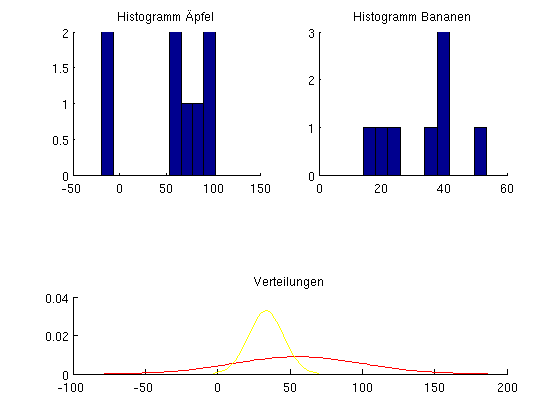
\includegraphics[width=1\linewidth]{plot.png}
  
  \caption{Training des Klassifikators für die jeweils 8 ersten Bilder. Die Accuracy der Klassifikation liegt bei 100\%. Charnoff liegt bei 0.0451 und Bhattacharyya bei 0.0556.}
\end{figure}
\newpage
\section{c}

Um nur jedes 10te Pixel zu übertragen bzw. zu betrachten sind nur geringfügige änderungen am Code vorzunehmen. Durch eine Modifikation der Schleifenbedingung der inneren
For-Schleife in \textbf{splitSegments2.m} wird erreicht, das für jede Zeile nur das 1,11,21...usw pixel betrachtet wird. Genauergesagt wird dadurch das Bild auf circa 
10\% seine Spalten reduziert. So wird zwar nicht exakt jedes 10. Pixel betrachtet (dazu müsste man einfach in den Schleifen mitzählen), aber so wird eine wesentlich
georndetere reduktion der Bandbreite gewährleistet. Man erhält also keien Pixelsalat, sondern ein quasi in der Breite runterskaliertes Bild.
\newline
Die Ergebnisse der Fehlerschranken liegen geringfügig unter den Fehlerschranken bei voller Bandbreite. Die Klassifikation zeigt auf den ersten Blick keine Veränderungen.
Als Fazit lässt sich also sagen, dass die Reduktion der Bandbreite keinen nennenswerten Qualitäts-Tradeoff darstellt und die eingesparte Rechenkapazität durchaus gerechtfertigt
erscheint. Interessant zu prüfen wäre an dieser Stelle in wiefern dadurch allerdings eine Zeitersparnis erreicht wird.
\newline
Mehr Aufschluss bringt ein Vergleich der Posterior Wahrscheinlichkeiten. Diese liegen sehr dicht beieinander. Die maximale Differenz beträgt 0.0033 und die mittlere
Differenz liegt bei 0.0013, bei einer Standardabweichung von 0.0012. Damit ist die Reduktion der Bandbreite offensichtlich unabhängig von der Qualität des Modells.
\begin{verbatim}
    Klassifikator1      Klassifikator2
    Apfel     Banane    Apfel     Banane
    0.9967    0.0033    0.9966    0.0034
    0.9988    0.0012    0.9989    0.0011
    1.0000    0.0000    1.0000    0.0000
    0.9800    0.0200    0.9833    0.0167
    0.9914    0.0086    0.9914    0.0086
    1.0000    0.0000    1.0000    0.0000
    0.6388    0.3612    0.6404    0.3596
    0.6099    0.3901    0.6109    0.3891
    0.2481    0.7519    0.2468    0.7532
    0.2393    0.7607    0.2404    0.7596
    0.2149    0.7851    0.2134    0.7866
    0.2218    0.7782    0.2227    0.7773
    0.2107    0.7893    0.2126    0.7874
    0.3613    0.6387    0.3583    0.6417
    0.4704    0.5296    0.4727    0.5273
    0.2358    0.7642    0.2392    0.7608
\end{verbatim}

\begin{figure}[htbp]
  \centering
    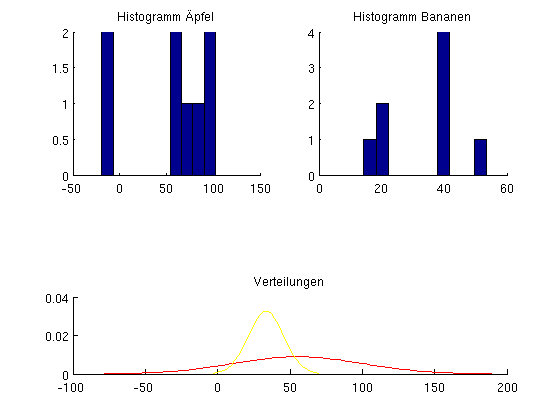
\includegraphics[width=1\linewidth]{plot2.png}
  
  \caption{Training des Klassifikators für die jeweils 8 ersten Bilder. Die Accuracy der Klassifikation liegt bei 100\%. Charnoff liegt bei 0.0437 und Bhattacharyya bei 0.0540.}
\end{figure}

\section{d}
Das Kreisfeature liefert bei der Erkennung geringfügig schlechtere Ergebnisse als der Rotanteil, allerdings wird der Killerapfel richtig erkannt. Wichtig für die Erkennung ist in diesem Fall besonders die richtige Segmentierung und damit die Wahl des richtigen Tresholds. (Siehe Abbildung 3)

\begin{figure}[htbp]
  \centering
    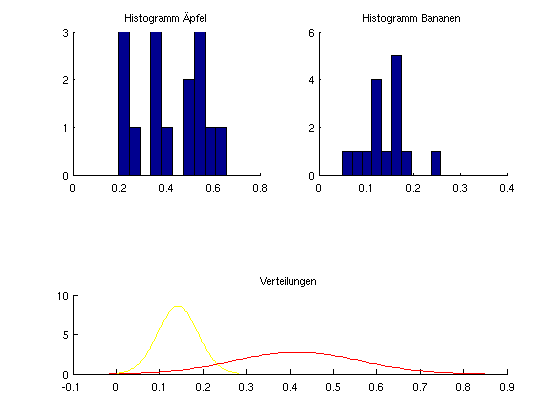
\includegraphics[width=1\linewidth]{plot3.png}
  
  \caption{Training des Klassifikators für alle Bilder. Die Accuracy der Klassifikation liegt bei 87\%. Charnoff liegt bei 0.4157 und Bhattacharyya bei 0.4197.}
\end{figure}

Die Reduktion der Datenmenge wird mit der Matlab-Methode \textbf{downsample} vorgenommen, das Graubild wird also praktisch in x-Richtung gestaucht. Trotz dieses offensichtlichen Nachteils liefert der reduzierte Ansatz sogar bessere Ergebnisse. (Siehe Abbildung 4)

\begin{figure}[htbp]
  \centering
    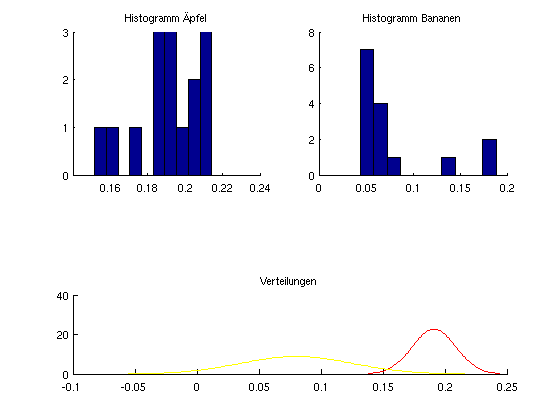
\includegraphics[width=1\linewidth]{plot4.png}
  
  \caption{Training des Klassifikators für alle Bilder. Die Accuracy der Klassifikation liegt bei 90\%. Charnoff liegt bei 0.4493 und Bhattacharyya bei 0.4510.}
\end{figure}

\section{e}
Beide Features zusammen ergeben wie erwartet ein relativ gutes Ergebniss. Der Killerapfel wird richtig zugeordnet.
\begin{figure}[htbp]
  \centering
    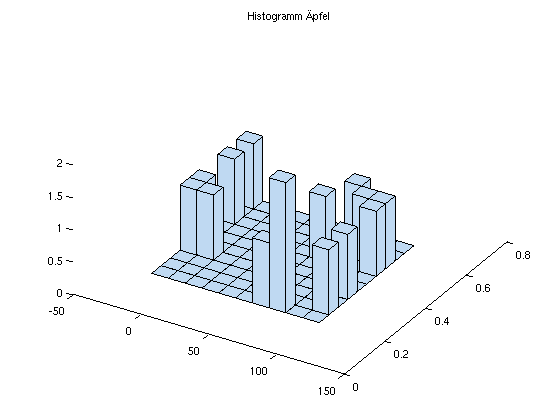
\includegraphics[width=1\linewidth]{plot5.png}
    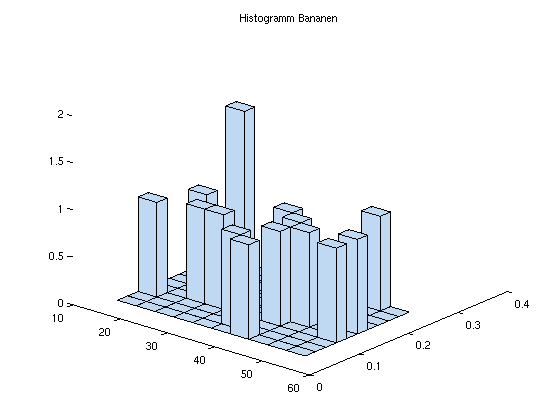
\includegraphics[width=1\linewidth]{plot6.png}
\end{figure}
\begin{figure}[htbp]
  \centering
    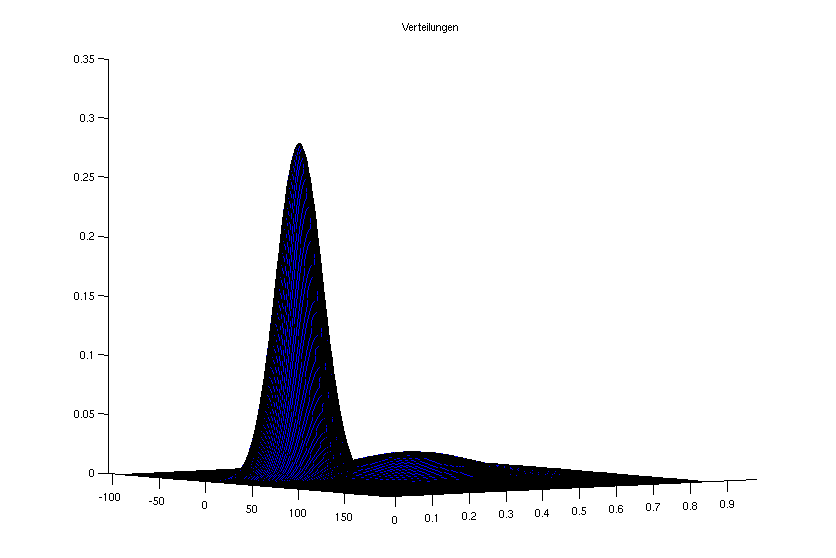
\includegraphics[width=1\linewidth]{plot7.png}
  \caption{Training des Klassifikators für alle Bilder. Die Accuracy der Klassifikation liegt bei 93\%.}
\end{figure}
\section{f}

Siehe \textbf{modifyClassifier.m}. 
\end{document}

